\documentclass[en]{pracamgr}

\usepackage{subcaption}
\usepackage{amsmath}
\usepackage{url}

\usepackage{tikz}
\usetikzlibrary{arrows.meta}
\tikzset{
    every node/.style={align=center,},
    tensor/.style={draw,rectangle,rounded corners,},
}

\usepackage{etoolbox}
\apptocmd{\thebibliography}{\raggedright}{}{}

\autor{Marcin Papierzyński}{345782}

\title{Music Style Transfer}
\titlepl{Transfer Stylu Muzycznego}

\kierunek{Computer Science}

\opiekun{dr hab. Marek Cygan\\
  Instytut Informatyki
  }

% miesiąc i~rok:
\date{October 2019}

%Podać dziedzinę wg klasyfikacji Socrates-Erasmus:
\dziedzina{11.4 Artificial Intelligence}

%Klasyfikacja tematyczna wedlug AMS (matematyka) lub ACM (informatyka)
\klasyfikacja{Applied computing\\
  Arts and humanities\\
  Sound and music computing}

\keywords{style transfer, music generation, midi, neural networks, recurrent neural networks, convolutional neural networks}

\newtheorem{defi}{Definicja}[section]

\begin{document}
\maketitle

%tu idzie streszczenie na strone poczatkowa
\begin{abstract}
    The goal of this work is to create a neural architecture that allows for creating a new arrangement of any song in the MIDI format, based on the style extracted from another song.
    I'm using an architecture based on LSTM layers as time-processing units, also utilizing convolutions.
    I define the notion of musical style and composition and train a model that is able to split and later merge them.
    This results in a symbolic music style transfer that supports a wide range of musical instruments and is in general much less restrictive than other most popular current solutions.
\end{abstract}

\tableofcontents
%\listoffigures
%\listoftables

\chapter{Introduction}

Transfer of style between images is a well-known problem.
Currently, it can be realized between any two images by using convolutional neural networks \cite{image_style_transfer}.
The analogous style transfer done for music is a much less explored topic and it is challenging even to define what exactly a musical style is.

\section{Goal statement}

In this paper the goal is to define some sensible notion of musical style and create a model that can create a different arrangement for any song based on style extracted from any other song.
The music used for training is assumed to be in the MIDI format and can use any range of instruments.
The instruments supported by the model must be set during training, but the supported styles do not -- we want the trained model to be able to extract style from any song.

Note that music generation is often done on raw waveform, most typically using spectrograms and frourier analyzis, as in \cite{music_generation}.
In this work however, I state the problem of music style transfer only concerning MIDI format for two reasons.

\begin{enumerate}
    \item Direct generating of realistically sounding music is in itself a hard problem, which I don't want to tackle here.
    \item
    MIDI format provides more structured data than raw sounds -- the input is divided as separate instruments, we have exact information about which notes are played when.
    Thus, working with MIDI files I can focus solely on the style transfer, which makes the task much easier.
\end{enumerate}

\chapter{Other works}

There exist previous works doing music style transfer to some extent.
A few examples are shortly described below.
All of them, however, are performing a simpler kind of a style transfer.

\section{Neural Translation of Musical Style}

In Neural Translation of Musical Style \cite{neural_translation} authors created a model than can learn to perform any given piano piece in either jazz or classical style.
The model does this by regression of notes' velocities (loudness), so it's effectively creating an interpretation of a given piano piece.
Therefore it's much simpler, because it only supports one instrument (piano) and cannot create a completely different arrangement.

\section{Symbolic Music Genre Transfer with CycleGAN}

In Symbolic Music Genre Transfer with CycleGAN \cite{cyclegan} the described model can create new arrangements but it can still only generate piano and the styles need to be set during training (in this case it's jazz, classic and pop).

\section{Play as You Like: Timbre-enhanced Multi-modal Music Style Transfer}

In Timbre-enhanced Multi-modal Music Style Transfer \cite{multimodal} the model can operate on different instruments, but the styles still need to be set during training (the styles are actually instruments, the authors are using guitar, piano and string quartet).
Like in the previous examples, it doesn't allow to transfer style between arbitrary songs.

\chapter{Overview and results}

\section{Musical style and composition}

For the musical style transfer, the two main notions concerning songs are composition and style.
I start by giving a rough definition of them.

Composition is any information about a song that is related to a specific moment in time, e.g. if the music gets louder or some instrument starts playing.
The most important part of a composition is the melody (played by one or more instruments).

The style, on the other hand, is information not related to any specific moment in time, e.g. the general mood of the song or the way specific instruments are used (for example, which instruments play the main melodic line and which ones create a backing).

Since music is a form of art, even though it can be understood and formally described, it will always be at least partly subjective.
This means that the exact way to split songs into composition and style is not unique (for example, used instruments may naturally be considered part of style, but they can also change in time).
The main assumption, however, is that composition-style splitting can be performed in \emph{some} fashion which can be learned by a complex enough model.

Since any song can be naturally interpreted as a time sequence, I will use a recurrent neural network as a model for splitting the input song into composition and style.
Composition, just like the input, is a time series, but simpler, with less features.
The style, on the other hand, is a single vector representing the whole song.
During training, the model splits the input song into composition and style, and then combines them to recreate the original song.
Because composition is much smaller than the input song, the model must include useful information in the style vector as well.

After training, I can use the model to extract style from a song and combine it with the composition extracted from another song.
The hypothesis is that this approach will allow for a sensible music style transfer.

\section{Results}

I've been able to achieve interesting results, resulting in a neural network that is able to create new arrangements of songs, as expected.
The exact characteristics of generated music varies, from very simple changes in used instruments, to generating a song that is almost unrecognizable from the original, but always souding like an actual music.
I consider the results to be satisfying, although there are some areas for further improvement -- the generated music sometimes doesn't sound completely natural, and the model is not providing an impressive style transfer for 

\chapter{Framework}

\section{Tools}

The whole project is implemented in Python.
The machine learning framework I use is PyTorch, along with mido -- a Python library for working with MIDI files.

\section{Data}

The dataset I use is Lakh MIDI Dataset\footnote{https://colinraffel.com/projects/lmd/}.
It contains over 100,000 songs in the MIDI format and covers various genres, including pop, rock or classical.

\chapter{Data flow}

The data flow of the whole architecture is composed of 3 stages: style extraction, predicting song information, and style application.

\section{Style extraction}

The input in the first stage is:
\begin{itemize}
    \item song information
    \begin{itemize}
        \item instruments used in a song
        \item mode of a song (major or minor)
        \item tempo (in beats per minute)
    \end{itemize}
    \item song content (information about which notes are played in any moment in time for any instrument used in a song)
\end{itemize}

Mode and used instruments are represented using one-hot encoding.
I use 41 most popular instruments in the dataset (percussion and 40 pitched instruments) covering 90\% of all the sounds in the dataset.
The tempo is a numerical value between 50 and 200 (and is clamped to that interval, if necessary).

The output is composed of 3 parts: melody, rhythm and style.
Each of them contains features as learnable embeddings.
I will refer to melody and rhythm as composition.

Melody should encode song content (like the input) but with no information about specific instruments (it must combine them).
It encodes all pitched instruments used in a song.

Rhythm contains additional information about the melody (but not explicitly related to specific notes) and features of percussion if it is present in the input song.
The main reason for introducing rhythm alongside melody is to be able to represent percussion (the only unpitched instrument) but at the same time do not force it if it's not present in the original song (the model should be able to add percussion to a song that originally didn't have it).

I require that there is always at least one pitched instrument used in a song, while the percussion is optional.
That way both melody and rhythm are always well-definied (there is at least one pitched instrument they can encode).

Melody and rhythm, along with the style, should enable to recreate all the instruments used in a song.

\section{Prediction of song information}

The input in this stage is style and rhythm.
The output is basic information about a song (as in the first stage):
\begin{itemize}
    \item used instruments (classification)
    \item mode (classification)
    \item tempo (regression)
\end{itemize}

All those outputs should coincide with the respective inputs from the first stage.
Note that the set of supported instruments can be arbitrarily large but needs to be specified during training.

\section{Style application}

At this stage the inputs are composition (i.e. melody and rhythm) and style from the first stage.
The output is the song content for each of the used instruments.
Generated song content should conincide with the input from the first stage.
In other words, the model must reconstruct the original song.
Figure \ref{fig:data_flow} depicts the data flow in all three stages.

\begin{figure}
    \centering
    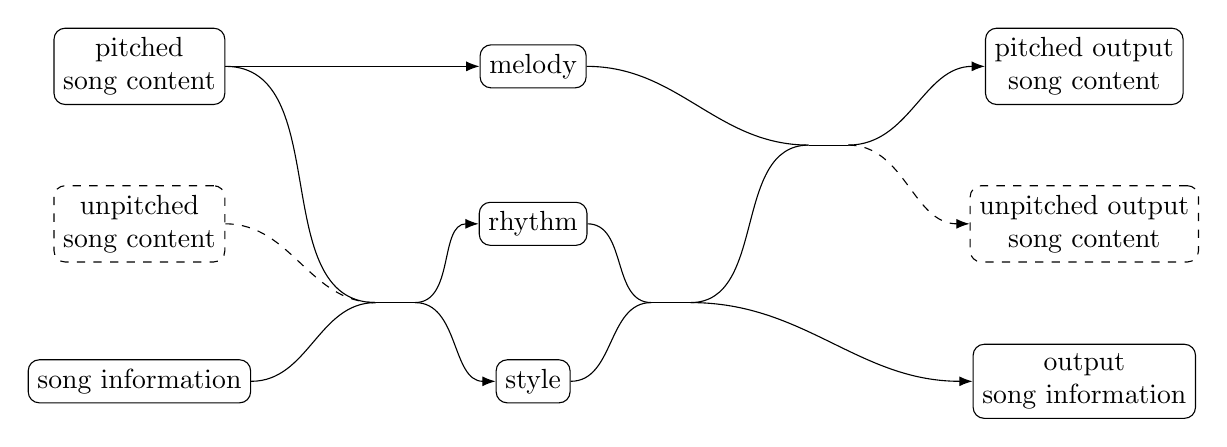
\begin{tikzpicture}
        \node[tensor] (pitched) at (0, 4) {pitched\\song content};
        \node[tensor, dashed] (unpitched) at (0, 2) {unpitched\\song content};
        \node[tensor] (info) at (0, 0) {song information};

        \coordinate (merge) at (3, 1);
        \coordinate (split) at (3.5, 1);

        \node[tensor] (melody) at (5, 4) {melody};
        \node[tensor] (rhythm) at (5, 2) {rhythm};
        \node[tensor] (style) at (5, 0) {style};

        \coordinate (merge2) at (6.5, 1);
        \coordinate (split2) at (7, 1);
        \coordinate (merge3) at (8.5, 3);
        \coordinate (split3) at (9, 3);

        \node[tensor] (pitched_output) at (12, 4) {pitched output\\song content};
        \node[tensor, dashed] (unpitched_output) at (12, 2) {unpitched output\\song content};
        \node[tensor] (output_info) at (12, 0) {output\\song information};

        \draw[-Latex] (pitched) to (melody);
        \draw (pitched) to [out=0,in=180] (merge);
        \draw[dashed] (unpitched) to [out=0,in=180] (merge);
        \draw (info) to [out=0,in=180] (merge);
        \draw (merge) to (split);
        \draw[-Latex] (split) to [out=0,in=180] (rhythm);
        \draw[-Latex] (split) to [out=0,in=180] (style);

        \draw (rhythm) to [out=0,in=180] (merge2);
        \draw (style) to [out=0,in=180] (merge2);
        \draw (merge2) to (split2);
        \draw (split2) to [out=0,in=180] (merge3);
        \draw (melody) to [out=0,in=180] (merge3);
        \draw[-Latex] (split2) to [out=0,in=180] (output_info);
        \draw (merge3) to (split3);
        \draw[-Latex] (split3) to [out=0,in=180] (pitched_output);
        \draw[-Latex, dashed] (split3) to [out=0,in=180] (unpitched_output);
    \end{tikzpicture}
    \caption{Data flow of the model (dashed parts are optional).}
    \label{fig:data_flow}
\end{figure}

\chapter{Data representation}

In MIDI format, the song is encoded as a sequence of events messages.
Messages can contain instructions like setting the tempo or playing a note.
Note events are assigned to one of the 16 channels -- each of those channels can represent a different instrument.

\section{MIDI encoding}

The MIDI file is encoded as a tensor in the format:
\begin{center}
    (\emph{batch, channel, bar, beat, beat fraction, note, note features}).
\end{center}

The \emph{channel} dimension refers to a MIDI channel (an instrument).
The \emph{bar}, \emph{beat} and \emph{beat fraction} dimensions point to the exact moment in a song when the note is being played.

\subsection{Specifying time}

I assume that the time signature cannot change, so that the number of the beats is constant throughout the song (usually 3 or 4).
The \emph{bar} and \emph{beat} dimensions denote in which bar and at which beat the note should play.
The \emph{beat fraction} dimension is specifying the exact moment during the beat.

I divide the beat into 8 parts, which gives 8 possible fractions: $0, \frac{1}{8}, \frac{2}{8}, \ldots, \frac{7}{8}$.
Independently, I also divide the beat into 3 parts: $0, \frac{1}{3}, \frac{2}{3}$.
Combining it, symplifying and sorting, we get 10 different fractions:
$$
0, \frac{1}{8}, \frac{1}{4}, \frac{1}{3}, \frac{3}{8}, \frac{1}{2}, \frac{5}{8}, \frac{3}{4}, \frac{2}{3}, \frac{7}{8}.
$$

Each \emph{note fraction} coordinate represents one of those fractions.
A single beat most commonly has length of a quarter note, which means that fractions with denominator 8 allow to represent up to 32th notes.
While division into powers of 2 is the most common in music, many songs also use division into three parts, called triplets.
Inclusion of fractions with denominator 3 allows for the exact representation of them, which otherwise would need to be approximated using fractions with denominator 8.
More fractions could be added to allow for representing faster melodies, but these 10 are enough for most songs.

The typical way of splitting the beat in neural music generation is to simply divide it into timesteps of equal length, e.g. into 12 parts \cite{clara}.
The downside of this approach is that it creates many "unnecessary" fractions (like $\frac{1}{12}$), which are not typically used, so they mainly only increase the size of the MIDI file representation.
The increase in the size is quite significant, since being able to represent 32th notes using this approach would require denominator $24=3\cdot8$, resulting in the whole input being over two times bigger.
Here I only introduce the fractions that are necessary to represent triplets ($\frac{1}{3}$ and $\frac{2}{3}$), omitting the rest.

The proposed approach also scales well with addition of more tuplets.
For example, adding support for quintuplets (division into 5 parts) would only require adding 4 more fractions ($\frac{1}{5}, \frac{2}{5}, \frac{3}{5}$ and $\frac{4}{5}$), resulting in a constant increase in size ($14=10 + 4$ timesteps), while the traditional approach would mean a 5-fold increase in the total size ($120=3\cdot5\cdot8$ timesteps). More complex tuplets are however much less common (and virtually never used in popular music), so I don't use them here.

It's worth noting that in my approach resulting fractions are not equidistant, meaning that it's not justified to apply convolution along the \emph{note fraction} dimension.
However, the length of this dimension is not substantial and it's still possible to apply convolution along \emph{bar} and \emph{beat} dimensions, so it's not a big limitation.

\subsection{Note features}

The above format is used for both percussion and pitched instruments.
However, the number of notes and note features (lengths of dimensions \emph{note} and \emph{note features} respectively) is different for percussion and for pitched instruments, so two tensors must be used: one for pitched instruments and one (possibly empty) for percussion.

Note features for pitched instruments are:
\begin{itemize}
    \item velocity (loudness)
    \item duration
    \item accidentals (raise or lower the note one semitone)
\end{itemize}

Accidentals are represented using one-hot encoding with vector of length 3 (raise the note, lower the note, or play the note unmodified), which gives a total of 5 features per note for pitched instruments.
For percussion the only note features are velocity and duration, which gives 2 features per note.

\section{Notes representation}

I use note's span of 8 octaves, each with 12 sounds, which gives 96 possible notes in total.
The notes are represented as one-hot encoded vectors with a slight modification.
In the standard one-hot encoding, each coordinate in a \emph{note} dimension would correspond to a specific note (so \emph{note} dimension would have length 96).
However, this way of encoding would pose a problem for style transfer.
Namely, depending on the mode of the song (major or minor), a different set of notes is used.
This means that the same song in a different mode would use different sounds in its melody.
Hence, with the typical way of encoding notes, the melody representation would partially impose style, which is not desired, since we want to split them.

To remedy that, I encode the notes relative to the scale the song is in.
Effectively, what is encoded are not the actual notes, but rather the scale degrees they represent; so the note C in a song in C major would be encoded the same way as the note G in a song in G minor.
That way, changing the scale of the song will not affect the melody representation.

This way of encoding only allows to encode notes contained in a given scale (which covers 7 out of 12 notes in each octave).
For example, if the song is in C major, we could only encode "white keys".
To allow for encoding all the remaining notes as well, each note has additional features (called accidentals) that can raise it or lower it one semitone.
Then we can represent all 12 notes in each octave.

The downside of this solution is that it requires the scale of the song to be known -- and finding it is in itself not a trivial problem.
I use fairly simple heuristics based on the Krumhansl-Schmuckler key-finding algorithm\footnote{http://rnhart.net/articles/key-finding/}, which predicts the scale of the song based on the frequency of notes used.

\section{Style and composition representation}

Melody is a tensor of shape
\begin{center}
    (\emph{batch, channel, bar, beat, beat fraction, note, features}),
\end{center}
which is the same as the input shape but with no \emph{instrument} dimension.
The number of note features may also be different.

Rhythm is a tensor of shape
\begin{center}
    (\emph{batch, channel, bar, beat, beat fraction, features}).
\end{center}
It's also similar to the input but this time with no \emph{instrument} and no \emph{note} dimensions.

Style is encoded as a regular vector, so it has shape
\begin{center}
    (\emph{batch, features}).
\end{center}

The number of features in a melody should be low enough so that the model cannot simply remember all the instruments in the input.
Instead, the model will need to learn some compressed high-level representation of the melody, from which it will later be able to reconstruct the input instruments, using the style vector.

\chapter{Model}

\section{Notation}

The nodes represent tensors, while the edges represent neural network layers -- standard fully-connected and activation layers, unless specified otherwise.
Leaky ReLUs are used as activation functions.

The $\oplus$ symbol is used to indicate elementwise addition (with broadcasting), and the $++$ symbol indicates concatenation of tensors.
Since the concatenated tensors often have different shapes, the concatenation is also performed with broadcasting.

\section{Model description}

Figure \ref{fig:style_extraction_model} shows the architecture of the model components in the style extraction stage.
The first step is encoding the input song content using convolutional and LSTM layers (figure \ref{fig:channels_encoder}).
The convolution is applied along the \emph{note} dimension, with stride equal to 7 (the number of scale degrees in a single octave).
This way, the output of the convolutional layer contains information about specific octaves in the song.
Afterwards, two hierarchical LSTM layers are used for further processing.
The first LSTM layer is applied along the \emph{beat} dimension (for each bar independently, with beats as timesteps), and the second one along the \emph{bar} dimension.
They produce the embedding of the song content which is passed to further submodules.

Style encoder uses an LSTM layer to process the generated embedding into a single time-independent vector (figure \ref{fig:style_encoder}).
Melody and rhythm encoders use both the original content and the generated embedding to produce the output (figures \ref{fig:melody_encoder} and \ref{fig:rhythm_encoder}).
The two-headed arrow represents a note generating submodule, shown in figure \ref{fig:generating_notes}.

\begin{figure}
    \centering
    \subcaptionbox{
        MIDI channels encoder.
        The convolution is applied along the \emph{note} dimension, independently for every beat.
        The first LSTM is applied for beats and the second one for bars.
        \label{fig:channels_encoder}
    }{
        \centering
        \resizebox{.47\linewidth}{!}{
            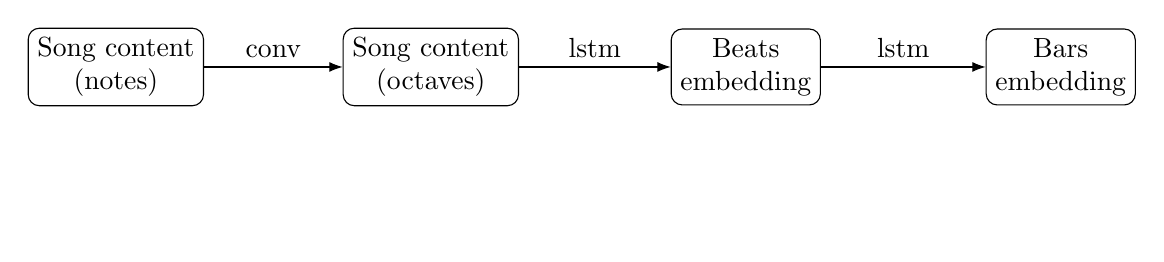
\begin{tikzpicture}
                \node[tensor] (notes_content) at (0, 2) {Song content\\(notes)};
                \node[tensor] (octaves_content) at (4, 2) {Song content\\(octaves)};
                \node[tensor] (beats) at (8, 2) {Beats\\embedding};
                \node[tensor] (bars) at (12, 2) {Bars\\embedding};

                \node (x) at (0, 0) {};

                \path (notes_content) edge[-Latex] node[above] {conv} (octaves_content);
                \path (octaves_content) edge[-Latex] node[above] {lstm} (beats);
                \path (beats) edge[-Latex] node[above] {lstm} (bars);
            \end{tikzpicture}
        }
    }\hfill%
    \subcaptionbox{
        Style encoder.
        \label{fig:style_encoder}
    }{
        \centering
        \resizebox{.47\linewidth}{!}{
            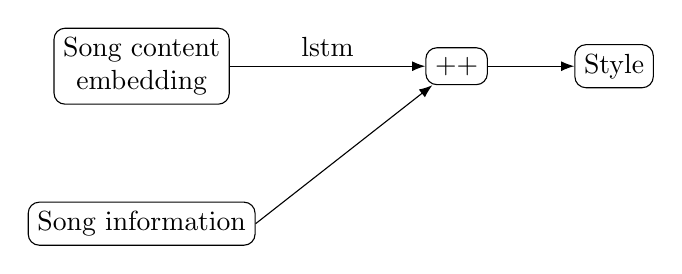
\begin{tikzpicture}
                \node[tensor] (bars) at (0, 2) {Song content\\embedding};
                \node[tensor] (info) at (0, 0) {Song information};

                \node[tensor] (concat) at (4, 2) {$++$};

                \node[tensor] (style) at (6, 2) {Style};

                \path (bars.east) edge[-Latex] node[above] {lstm} (concat);
                \draw[-Latex] (info.east) to (concat);

                \draw[-Latex] (concat) to (style);
            \end{tikzpicture}
        }
    }
    \subcaptionbox{
        Melody encoder.
        \label{fig:melody_encoder}
    }{
        \centering
        \resizebox{.47\linewidth}{!}{
            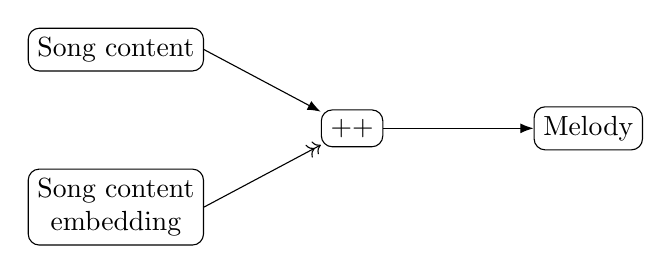
\begin{tikzpicture}
                \node[tensor] (content) at (0, 3) {Song content};
                \node[tensor] (content_emb) at (0, 1) {Song content\\embedding};
        
                \node[tensor] (concat) at (3, 2) {$++$};
        
                \node[tensor] (melody) at (6, 2) {Melody};
        
                \draw[-Latex] (content.east) to (concat);
                \draw [->>] (content_emb.east) to (concat);
        
                \draw[-Latex] (concat) to (melody);
            \end{tikzpicture}
        }
    }\hfill%
    \subcaptionbox{
        Rhythm encoder.
        \label{fig:rhythm_encoder}
    }{
        \centering
        \resizebox{.47\linewidth}{!}{
            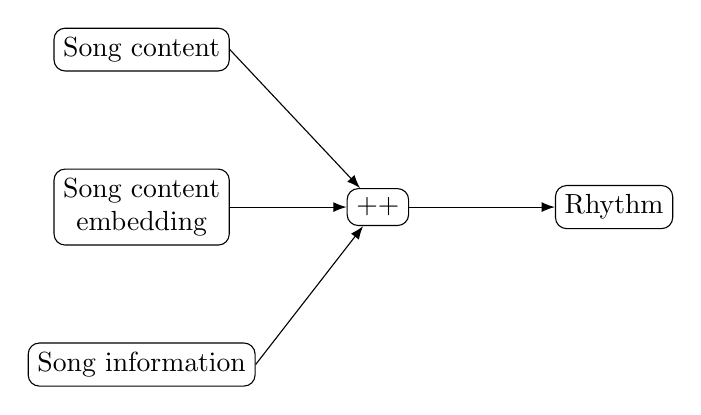
\begin{tikzpicture}
                \node[tensor] (content) at (0, 4) {Song content};
                \node[tensor] (content_emb) at (0, 2) {Song content\\embedding};
                \node[tensor] (info) at (0, 0) {Song information};
        
                \node[tensor] (concat) at (3, 2) {$++$};
        
                \node[tensor] (rhythm) at (6, 2) {Rhythm};
        
                \draw[-Latex] (content.east) to (concat);
                \draw[-Latex] (content_emb.east) to (concat);
                \draw[-Latex] (info.east) to (concat);
        
                \draw[-Latex] (concat) to (rhythm);
            \end{tikzpicture}
        }
    }
    \caption{Style extraction stage.}
    \label{fig:style_extraction_model}
\end{figure}

\begin{figure}
    \centering
    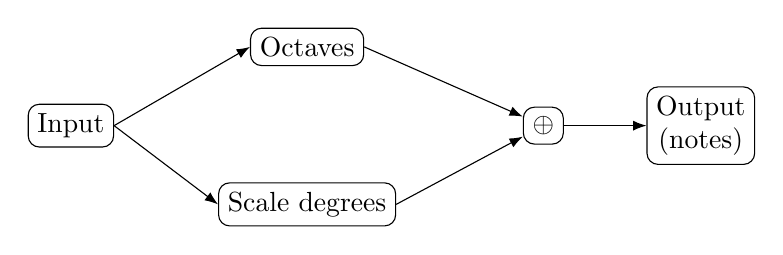
\begin{tikzpicture}
        \node[tensor] (input) at (0, 2) {Input};

        \node[tensor] (octaves) at (3, 3) {Octaves};
        \node[tensor] (scale_degrees) at (3, 1) {Scale degrees};

        \node[tensor] (plus) at (6, 2) {$\oplus$};

        \node[tensor] (output) at (8, 2) {Output\\(notes)};

        \draw[-Latex] (input.east) to (octaves.west);
        \draw[-Latex] (input.east) to (scale_degrees.west);

        \draw[-Latex] (octaves.east) to (plus);
        \draw[-Latex] (scale_degrees.east) to (plus);

        \draw[-Latex] (plus) to (output);
    \end{tikzpicture}
    \caption{
        A submodule used for generating notes.
        It generates octave-specific and scale degree-specific information separately, before merging them.
        Such architecture allows the generated notes to depend on the exact octave, while still preserving correlation between different octaves.
    }
    \label{fig:generating_notes}
\end{figure}

Figure \ref{fig:final_stages} shows model architecture in the final two stages.

\begin{figure}
    \centering
    \subcaptionbox{
        Song information model.
        \label{fig:a}
    }{
        \resizebox{.47\linewidth}{!}{
            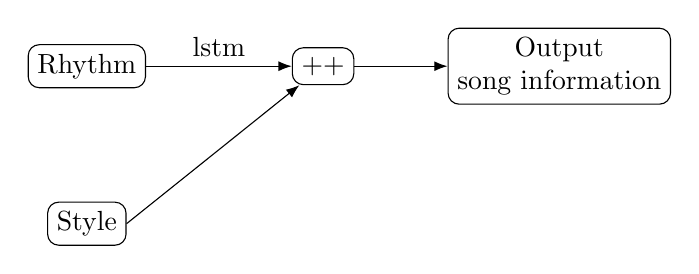
\begin{tikzpicture}
                \node[tensor] (rhythm) at (0, 2) {Rhythm};
                \node[tensor] (style) at (0, 0) {Style};
        
                \node[tensor] (concat) at (3, 2) {$++$};
        
                \node[tensor] (output_info) at (6, 2) {Output\\song information};
        
                \path (rhythm.east) edge[-Latex] node[above] {lstm} (concat);
                \draw[-Latex] (style.east) to (concat);
        
                \draw[-Latex] (concat) to (output_info);
            \end{tikzpicture}
        }
    }\hfill%
    \subcaptionbox{
        Style applier.
        \label{fig:b}
    }{
        \resizebox{.47\linewidth}{!}{
            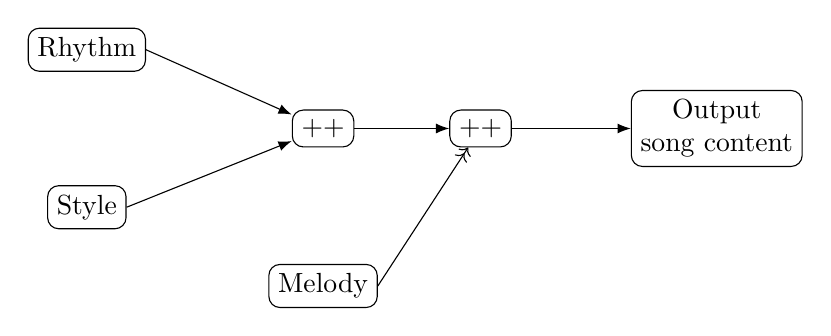
\begin{tikzpicture}
                \node[tensor] (style) at (0, 1) {Style};
                \node[tensor] (rhythm) at (0, 3) {Rhythm};
        
                \node[tensor] (concat) at (3, 2) {$++$};
                \node[tensor] (melody) at (3, 0) {Melody};
        
                \node[tensor] (concat2) at (5, 2) {$++$};
        
                \node[tensor] (output) at (8, 2) {Output\\song content};
        
                \draw[-Latex] (rhythm.east) to (concat);
                \draw[-Latex] (style.east) to (concat);
        
                \draw[-Latex] (concat) to (concat2);
                \draw [->>] (melody.east) to (concat2);
        
                \draw[-Latex] (concat2) to (output);
            \end{tikzpicture}
        }
    }
    \caption{Song information prediction (\ref{fig:a}) and style application (\ref{fig:b}) stages.}
    \label{fig:final_stages}
\end{figure}

\section{Melody and rhythm size}

The most important hyperparameters in this architecture are melody and rhythm embedding sizes, which were set to values 8 and 32 respectively.
Recall that the number of features per note for pitched instruments is equal to 5, which means that
the melody has a slightly bigger size than a single pitched instrument (but needs to encode \emph{all} pitched instruments used in a song).
The melody contains embedding for each note, as opposed to the rhyhm, so the size of the rhythm embedding can be set to a higher value than the melody.

Increasing the size of the melody and/or rhythm embeddings would lead to a better reconstruction of songs but a worse style transfer, since the model could then easily overfit by remembering more features in the composition, effectively ignoring the style vector.
Thereforce, composition embeddings should be kept rather small for this architecture, to prevent overfitting.

\chapter{Experiments}

\section{Loss function}

The loss function measures if the song generated by the model is the same as the input song. It is defined as a combination of many components, with the following structure:
\begin{itemize}
    \item total loss
	\begin{itemize}
	    \item channels loss
		\begin{itemize}
			\item pitched channels loss
            \begin{itemize}
                \item notes loss (complement of smooth F1 score)
                \item velocity loss (MSE)
                \item duration loss (MSE)
                \item accidentals loss (cross-entropy)
            \end{itemize}
			\item unpitched channels loss
            \begin{itemize}
                \item notes loss (complement of smooth F1 score)
                \item velocity loss (MSE)
                \item duration loss (MSE)
            \end{itemize}
		\end{itemize}
        \item song information loss
        \begin{itemize}
            \item instruments loss (cross-entropy)
            \item tempo loss (MSE)
            \item mode loss (cross-entropy)
        \end{itemize}
	\end{itemize}
\end{itemize}

This hierarchy signifies that the total loss is the average of channels loss and song information loss, channels loss is the average of pitched and unpitched channels loss, etc.

Notes loss is measuring if the model is generating the right sounds.
Since the desired output is greatly unbalanced (most of all the possible notes will not be played), I'm using a complement of smooth F1 score to measure notes loss:
\nopagebreak

\begin{equation}
    \textrm{notes loss} = 1 - F_1.
\end{equation}

Smooth $F_1$ score is definied in a standard way, using
\nopagebreak
\begin{align}
    & \textrm{true positive} = \min(p, t), \\
    & \textrm{false positive} = \max(0, p - t), \\
    & \textrm{false negative} = \max(0, t - p),
\end{align}

where $p,t\in[0,1]$ are prediction and ground truth respectively, interpreted as fuzzy logical values.
In case when $p$ and $t$ can only take discrete values of 0 or 1, this gives a standard definition of the $F_1$ score.
Thus, it is a generalization of the $F_1$ score compatible with gradient descent.
In our case the notes' fuzzy logical values are defined from velocity (1 meaning that the note is played with maximum possible velocity, and 0 meaning that the note is not played at all).

Velocity loss measures if the model is generating notes with the right loudness.
Velocity is already measured by the notes loss (acquiring maximum $F_1$ score requires playing with exactly right velocities), so this loss function provides additional, more explicit component measuring the velocity error.
It only takes into account the notes that should be played to avoid problems with unbalanced output (the same is true for duration loss).

Since different kinds of loss functions have different magnitudes, before averaging, all the components are normalized to take values in the $[0,1]$ interval.
Then, the normalized components are averaged using quadratic mean to yield the total loss. The use of quadratic mean instead of arithmetic promotes minimizing the components that have the greatest value, resulting in a more balanced training.

\section{Training}

The model was trained for 5000 iterations using the Adam optimizer \cite{adam}.
In each iteration the input is a random song from the dataset.
Figure \ref{fig:total} shows total loss during training, while figures \ref{fig:channels} and \ref{fig:song_info} show specific components of the loss function.
All the plots are smoothed using exponential moving average with momentum parameter equal to .99 and initial bias equal to 1 (i.e. maximum possible error).

\begin{figure}
    \centering
    \subcaptionbox{Total loss.}{
        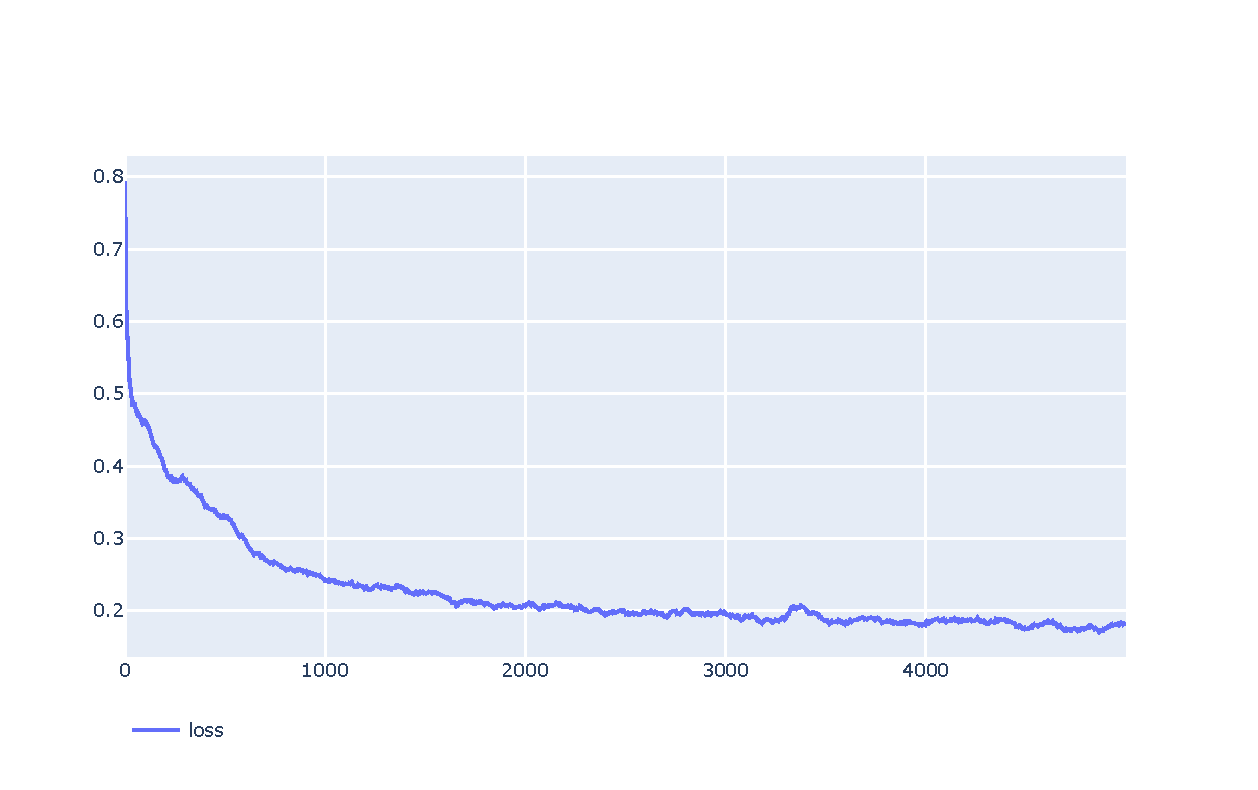
\includegraphics[width=.48\linewidth]{figures/training.pdf}
    }%
    \subcaptionbox{Loss components.}{
        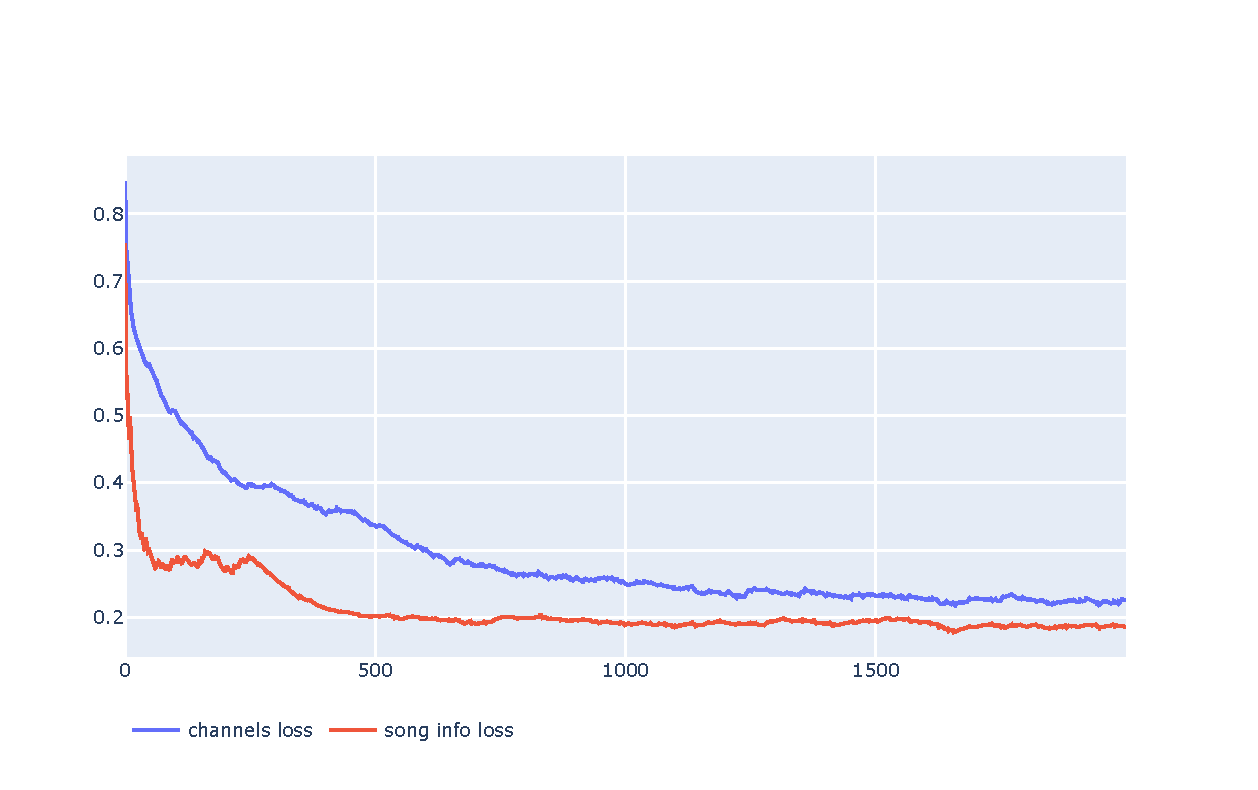
\includegraphics[width=.48\linewidth]{figures/total.pdf}
    }
    \caption{Total loss and its components during training.}
    \label{fig:total}
\end{figure}

Figure \ref{fig:pitched_vs_unptiched} shows how pitched and unpitched notes losses compare during trainig.
We can see that the model needs around 100 iterations to start learning pitched instruments (with the pitched notes barely below 1), during which time the unpitched loss is already significantly lower (around .7).
This can be explained by the fact that percussion is in general more repetitive than pitched instruments, so it's possible to achieve that level of the unpitched loss by mostly repeating the most common drum patterns.
This hypothesis can be confirmed by listening to the music generated by the snapshot of the model near the beginning of the training (for example at the iteration 300, when the unpitched notes loss shortly flattens at the level of .7).
As it turns out, the generated percussion is indeed very basic, featuring only some typical drum patters found in most of the pop/rock music.
The fully-trained model can nevertheless generate percussion that is relatively complex.

\begin{figure}
    \centering
    \subcaptionbox{
        Pitched loss components.
        The notes loss measures if the model is playing the right notes, while other components measure the specific features of the played notes.
        The notes loss eventually saturates at around .45 (giving $F_1$ score of .65).
    }{
        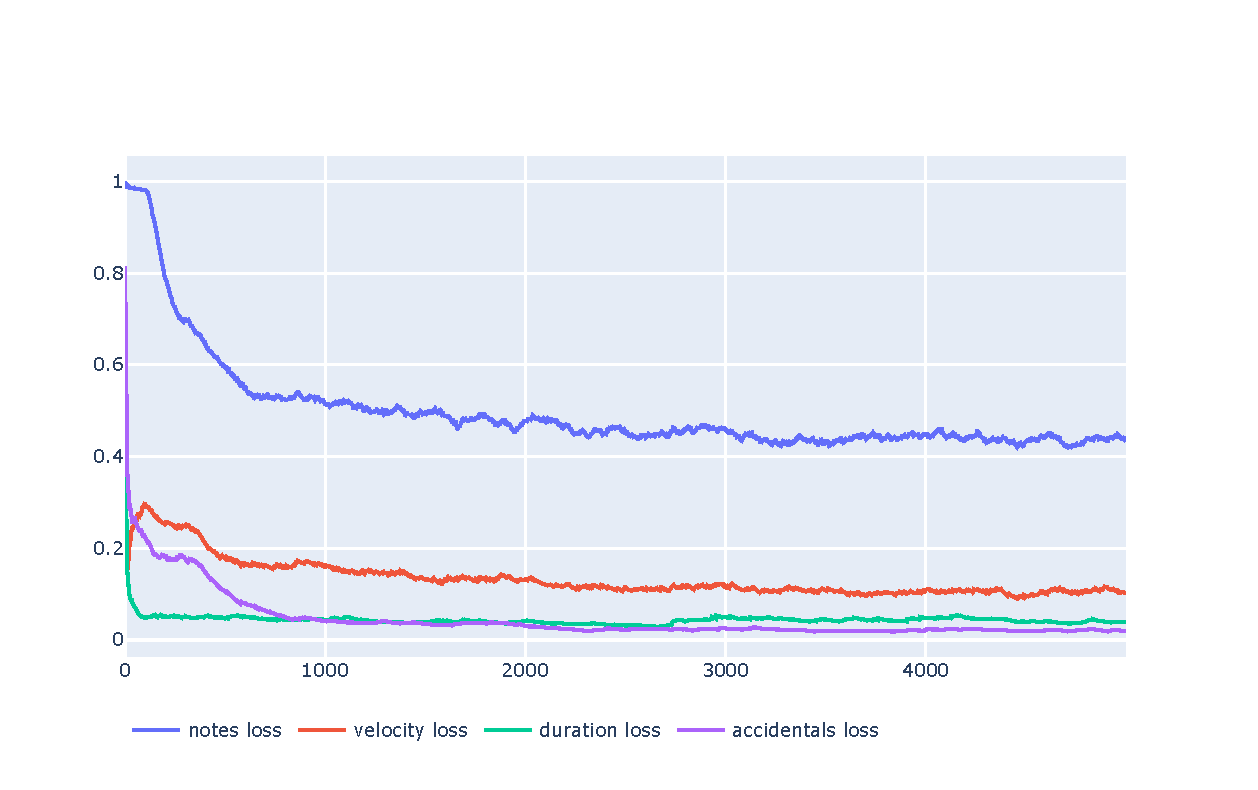
\includegraphics[width=.95\linewidth]{figures/pitched.pdf}
    }
    \subcaptionbox{
        Comparision of pitched and unpitched notes loss.
        The red line represents how well the model is playing the percussion, while the blue line represents all the other instruments.
        We can see that in general pitched instruments are harder than percussion.
        There are however a few hundred iterations during training when the model is actually slightly better at playing pitched instruments than percussion.
        \label{fig:pitched_vs_unptiched}
    }{
        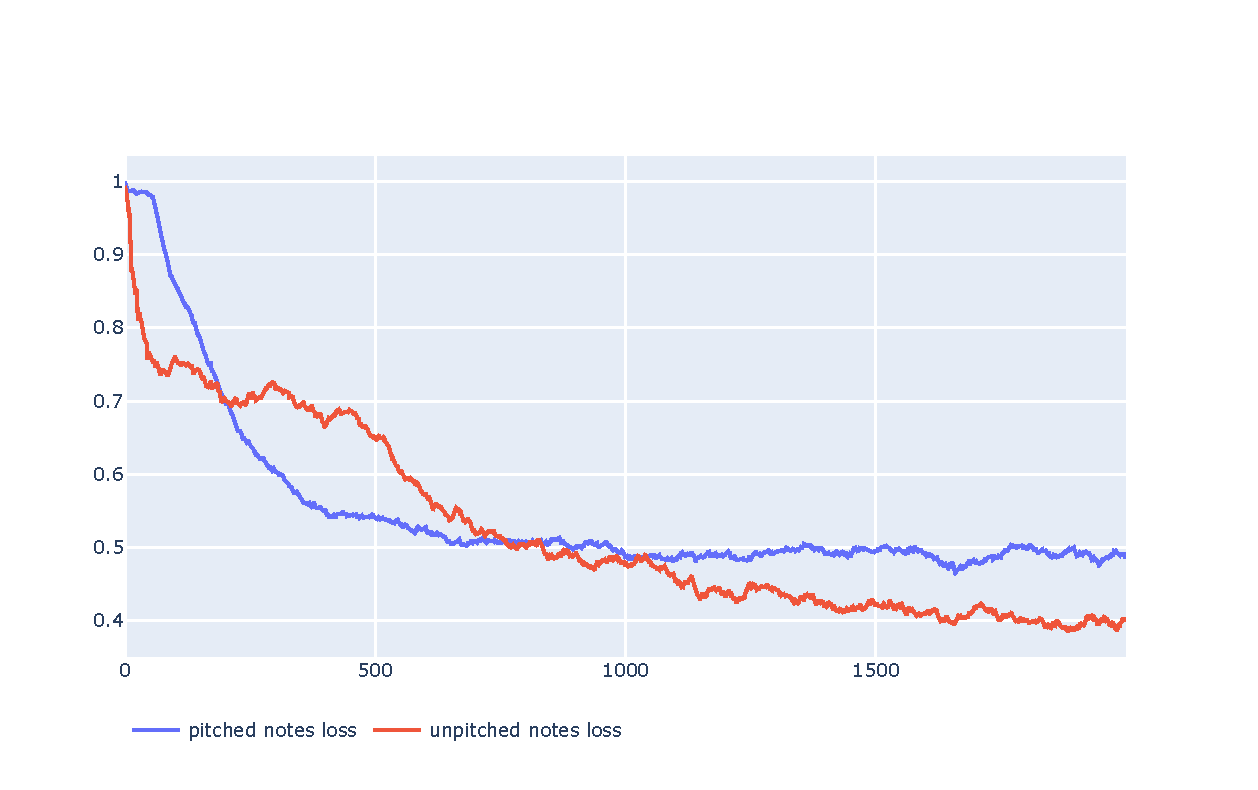
\includegraphics[width=.95\linewidth]{figures/notes.pdf}
    }
    \caption{Channels loss during training.}
    \label{fig:channels}
\end{figure}

\begin{figure}
    \centering
    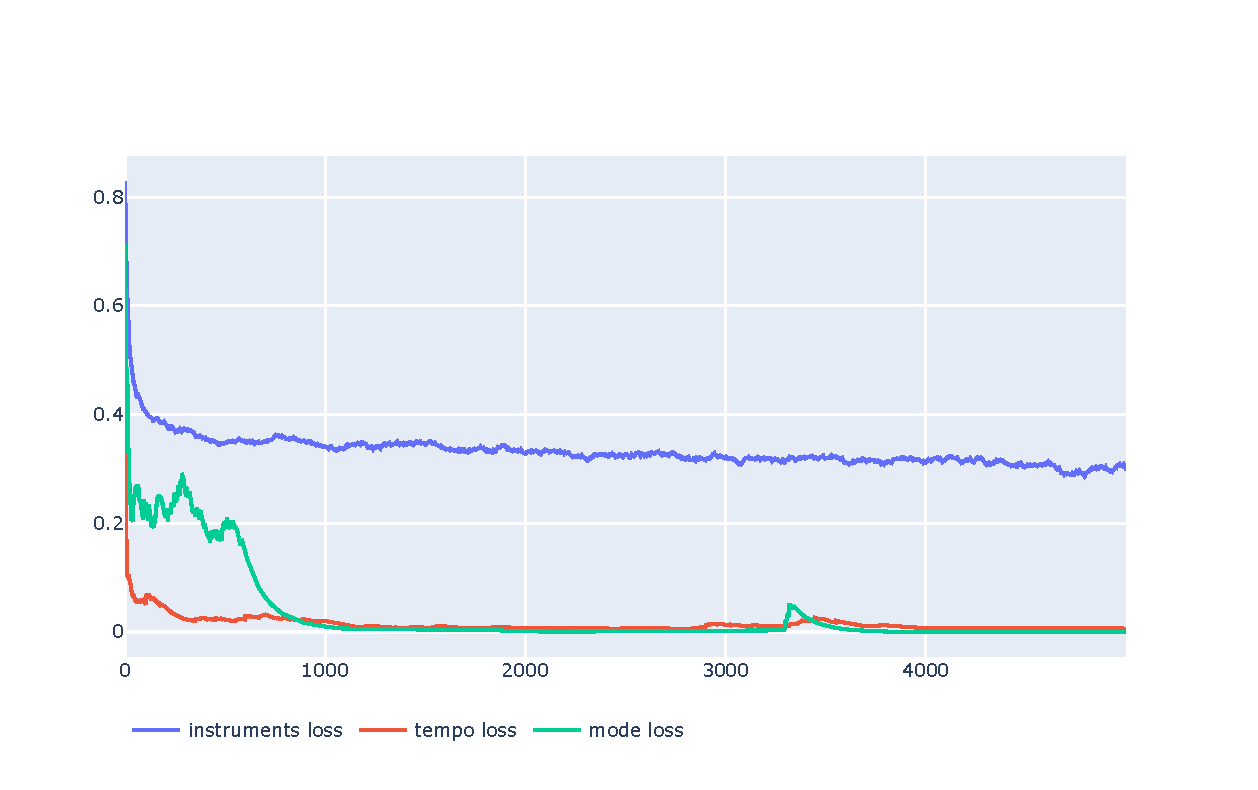
\includegraphics[width=\linewidth]{figures/song-info.pdf}
    \caption{Song information loss components during training.}
    \label{fig:song_info}
\end{figure}

\section{Reconstructing the song}

The neural network can fairly easy reconstruct the song in a way that is immediately recognizable, although often with some differences.
It's very common for the model to change the exact instrument that is playing some part, for example changing an electric guitar to an acoustic one, or even piano to guitar, especially if there are many instruments used in the song.
These are not a big problems for the style transfer, however, since changing the original song is our goal.

\section{Style transfer}

The trained model can be used to transfer style between songs.
To do this, the model needs to extract the composition from one song and the style from the other.
Then, the resulting composition and style are used to predict song information (i.e. mode, tempo and used instruments) and generate the content of the predicted instruments.

The first, most obvious application is to do the exact same thing as for the image style transfer, i.e. having two songs transfer the style from one to the other.
It can be done both ways at once, therefore doing a "style switch": generating song A in a style of song B, and song B in a style of song A.
In practice however it's much more informative to apply different styles to the same song, to see how they compare.

I used various groups of usually four songs (one for composition and three as style sources) to test the style transfer.
The quality of the results varies depending on the exact songs.
In some cases the generated music sounds unnatural, with a sudden changes in loudness, but in other instances the results are quite naturally-sounding.
For some songs the style transfer is mostly switching tempo and using different instruments for melody, but there are cases when it creates a completely differently sounding arrangement.

% \subsection{One instruments vs. many instruments}


\begin{thebibliography}{99}
\addcontentsline{toc}{chapter}{Bibliography}

\bibitem{image_style_transfer} Leon A. Gatys, Alexander S. Ecker, Matthias Bethge, \textit{Image Style Transfer Using Convolutional Neural Networks}, \url{https://www.cv-foundation.org/openaccess/content_cvpr_2016/papers/Gatys_Image_Style_Transfer_CVPR_2016_paper.pdf}.

\bibitem{music_generation} Piotr Kozakowski, Bartosz Michalak, \textit{Music generation using artificial neural networks}.

\bibitem{neural_translation} Iman Malik, Carl Henrik Ek, \textit{Neural Translation of Musical Style}, \url{https://arxiv.org/abs/1708.03535}.

\bibitem{cyclegan} Gino Brunner, Yuyi Wang, Roger Wattenhofer, Sumu Zhao, \textit{Symbolic Music Genre Transfer with CycleGAN}, \url{https://arxiv.org/abs/1809.07575}.

\bibitem{multimodal} Chien-Yu Lu, Min-Xin Xue, Chia-Che Chang, Che-Rung Lee, Li Su, \textit{Play as You Like: Timbre-enhanced Multi-modal Music Style Transfer}, \url{https://arxiv.org/abs/1811.12214}.

\bibitem{clara} Christine Payne, OpenAI Scholars Program, \textit{Clara: Generating Polyphonic and Multi-Instrument Music Using an AWD-LSTM Architecture}, \url{http://www.christinemcleavey.com/files/clara-musical-lstm.pdf}.

\bibitem{adam} Diederik P. Kingma, Jimmy Ba, \textit{Adam: A Method for Stochastic Optimization}, \url{https://arxiv.org/abs/1412.6980}.

\end{thebibliography}

\end{document}
